\FloatBarrier
\subsection{Implementazione dei canali con memoria condivisa}
\label{sct:specifica_sm}
Sfruttando la memoria condivisa si ha una implementazione semplice e lock-free delle comunicazioni simmetrica e asimmetrica con il protocollo Rdy-Ack. Ci\`o \`e determinato dal fatto che non esiste un buffer o altre strutture dati sulle quali i processi devono accedere in modo indivisibile. L'adozione di un grado di asincronia unitario e la sincronizzazione tramite gli eventi Rdy e Ack permette di effettuare accessi al descrittore del canale senza la necessit\`a di mutua esclusione.

\subsubsection{Comunicazione simmetrica}
\label{sct:sym_sm_rdyack}
Si considera la comunicazione simmetrica: il descrittore di canale \`e costituito da tre informazioni:
\begin{inparaenum}[\itshape a~\upshape)] 
\item il valore di Rdy, \item il valore di Ack, \item il valore del messaggio.
\end{inparaenum}
Ogni informazione \`e allocata in una parola, in particolare abbiamo la seguente definizione del descrittore di canale:  i flag di Rdy e di Ack sono di tipo intero, il messaggio \`e di tipo riferimento.
\begin{lstlisting}
struct ch_sym_sm_rdyack_t { 
  int rdy; 
  int ack; 
  void *value;
};
\end{lstlisting}
La segnalazione di un evento di Rdy o di Ack avviene impostando al valore 1 il corrispondente campo nel descrittore di canale. L'attesa attiva di un processo sul canale \`e realizza con la strategia \emph{retry} sul valore del flag Rdy o Ack: si continua a testare il valore del flag fino a quando non assume valore 1.
Il protocollo di comunicazione viene perci\`o realizzato con le seguenti azioni:
\begin{lstlisting}[
        morekeywords={rdy, ack, value},
        caption={Descrizione astratta del protocollo di comunicazione Rdy-Ack su memoria condivisa},
        label={lst:abstr_mem_sym}
]       
send(ch_descr, msg) ::
  wait until ch_descr->ack flag is equal to 1;
  reset ch_descr->ack flag to 0;
  copy msg into ch_descr->value entry;
  memory_fence();
  set ch_descr->rdy flag to 1;

receive(ch_descr) ::
  wait until ch_descr->rdy flag is equal to 1;
  reset ch_descr->rdy flag to 0;
  read the ch_decsr->value entry;
  set ch_descr->ack flag to 1;
\end{lstlisting}
La mutua esclusione nell'uso del valore del canale da parte dei processi mittente e destinatario \`e garantita dalla sincronizzazione dei due processi sui due valori di Rdy e Ack: ogni processo accede al valore del canale solo dopo che il processo partner ha notificato tale possibilit\`a. Per garantire la correttezza della comunicazione \`e quindi sufficiente adottare la seguente condizione iniziale:
\begin{itemize}
\item all'avvio dell'applicazione tutti i canali devono avere descrittore con campo Ack inizializzato ad 1 e capo Rdy inizializzato a 0.
\end{itemize}
Tale condizione iniziale, insieme all'adozione del protocollo, garantisce la seguente propriet\`a:
\begin{itemize}
\item ogni notifica di evento Rdy o Ack trova sempre l'evento corrispondente precedentemente falso.
\end{itemize}

%% L'IMPLEMENTAZIONE \`E LOCK-FREE, NECESSARIA MEMORY FENCE
Il fatto che sia possibile evitare l'uso di meccanismi di lock per l'esecuzione indivisibile del codice \`e un aspetto positivo dell'implementazione con memoria condivisa del protocollo Rdy-Ack, in quanto si evitano i relativi overhead sulle prestazioni. Al fine di garantire la correttezza \`e tuttavia richiesto l'uso di scritture sincrone alla memoria condivisa. \`E necessario che le scritture effettuate dal mittente sul valore del canale e sul flag di Rdy siano viste dal destinatario nello stesso ordine. Come descritto in sezione~\ref{sct:intro_arch_memory}, \tile\ adotta un modello rilassato di consistenza della memoria, sia per quanto riguarda l'ordinamento di istruzioni all'interno di una CPU, sia per l'atomicit\`a delle scritture in memoria condivisa. Ci\`o rende necessario l'uso di una barriera di memoria tra le due scritture effettuate dal mittente (riga 5 del codice~\ref{lst:abstr_mem_sym}), in modo che la scrittura del valore 1 sul flag Rdy sia sempre vista dal processo destinatario dopo la scrittura del messaggio nel canale. Il comportamento sincrono delle scritture in memoria, indotto dall'uso della barriera, produce overheads aggiuntivi rispetto al comportamento asincrono delle scritture. La barriera della memoria, e la corrispondente degradazione delle prestazioni, pu\`o essere eliminata con l'adozione di un protocollo di comunicazione alternativo, come mostrato in sezione~\ref{sct:sym_sm_nullack}.

%% USO SEMPRE LA CACHE
La politica di attesa attiva \emph{retry} \`e caratterizzata da un aumento dei conflitti alla memoria principale. Per evitare ci\`o e ridurre la latenza di sveglia si prendono in considerazione solo implementazioni che fanno uso della gerarchia cache. In tale scenario la prima lettura del valore di un flag causa il trasferimento del blocco corrispondente nei livelli L2 e L1D della cache locale, e le letture successive del valore del flag rimangano interne alla CPU, in quanto servite dalla cache locale. Quando il processo partner esegue la scrittura sul flag il meccanismo di coerenza della cache provvede a notificare il cambiamento e aggiornare il valore nella cache locale.

%% EFFETTO SULLE PRESTAZIONI DELLA COERENZA CACHE
Come descritto in sezione~\ref{sct:intro_arch_cache} il meccanismo di coerenza della cache \`e configurabile in molti aspetti, in particolare \`e possibile impostare il PE Home per una certa pagina di memoria. 
In sezione~\ref{sct:intro_arch_cache} viene spiegato come l'uso della strategia \emph{Remote Homing} sia conveniente in computazioni con singolo consumatore di una struttura dati condivisa, e permetta di evitare l'uso di invalidazioni e conseguenti copie di blocchi.
%, consentendo invece l'attuazione di un modello di programmazione di tipo \emph{remote storing}. 
Di seguito descriviamo il comportamento della comunicazione simmetrica con il protocollo Rdy-Ack e il descrittore di canale presentati, con la configurazione predefinita della coerenza della cache, quindi verr\`a presentata una versione ottimizzata che minimizza i messaggi di coerenza e le copie dei blocchi grazie alla configurazione dei PEs Home e al partizionamento del descrittore del canale nelle cache dei PEs.

%% USO PREDEFINITO DELLA COERENZA CACHE
\begin{figure}[!t]
  \centering
  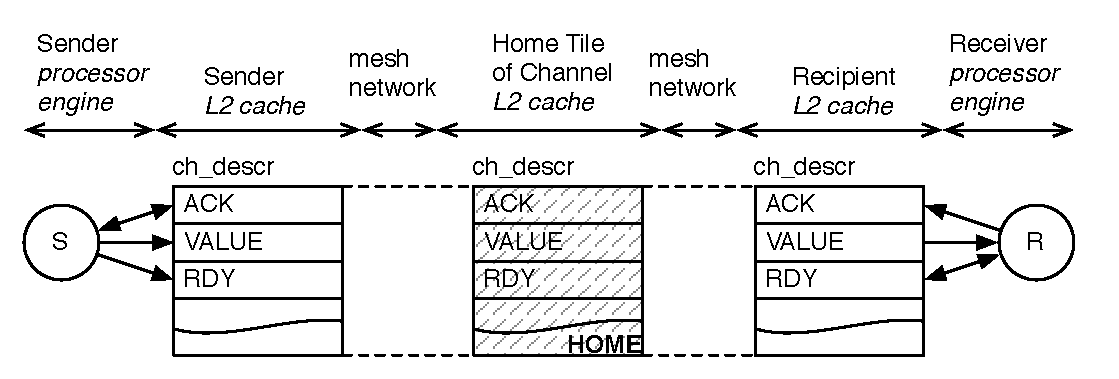
\includegraphics[scale=.5]{cache_sym_sm_no.pdf}
  \caption[Comunicazione simmetrica su memoria condivisa, non ottimizzata]{Rappresentazione di una comunicazione simmetrica tra un processo mittente $S$ e uno destinatario $R$ con uso della memoria condivisa e gestione predefinita della coerenza di cache (hash-for-home strategy)} 
  \label{fig:cache_sym_sm_no}
\end{figure}
La strategia predefinita di allocazione delle pagine di memoria nelle cache \`e \emph{Hash-for-Home} \cite{ug205}. La gestione delle informazioni di coerenza di cache, in particolare l'entrata della Directory, del blocco che contiene il descrittore di canale allocato viene affidata ad un generico processing element $\mathrm{PE}_k$. Durante l'esecuzione del programma parallelo il processo mittente, eseguito in $\mathrm{PE}_i$, e il processo destinatario, eseguito in $\mathrm{PE}_j$, eseguono, per mezzo delle primitive di comunicazione, degli accessi al descrittore di canale. In generale $k \neq i$ e $k \neq j$ quindi si hanno tre copie del blocco contenente il descrittore di canale come mostrato in figura~\ref{fig:cache_sym_sm_no}. La modifica di un campo del descrittore del canale effettuata da uno dei due processi comunicanti provoca l'invalidazione del blocco di L2 nel PE che esegue il processo partner. Quando il PE che contiene il blocco invalidato riferisce il descrittore di canale, l'intero blocco sar\`a trasferito dal PE Home, $\mathrm{PE}_k$, al PE stesso. Nel caso migliore si ha una invalidazione e corrispondente trasferimento di blocco al termine di ogni esecuzione di una primitiva di comunicazione, quando viene notificato un evento di sincronizzazione al processo partner per mezzo di una scrittura nel descrittore di canale.
%% USO OTTIMIZZATO DELLA COERENZA CACHE
\begin{table}[!b]
  \begin{center}
    \begin{tabular}{ | l | l | l | l |}
      \hline
      & Rdy & Ack & Value \\ \hline
      Sender & Write Only & Read and Write & Write Only \\
      Receiver & Read and Write & Write Only & Read Only \\
      \hline
    \end{tabular}
  \end{center}
  \caption[Modalit\`a di accesso ad un canale su memoria condivisa]{Modalit\`a di accesso ai campi del descrittore di canale su memoria condivisa}
  \label{tab:accessi_descr_ch}
\end{table}

Questo offre lo spunto su come ottimizzare l'uso delle cache: la scrittura sul campo del descrittore di canale che implementa un segnale di sincronizzazione dovrebbe essere inoltrata direttamente alla cache del PE che attende il segnale, evitando il trasferimento di un blocco di L2 per la trasmissione di una sola parola. 
%Tale comportamento \`e simile al modello di Remote Store Programming nel quale un processo pu\`o scrivere nella memoria locale di un altro processo.
Questo comportamento \`e possibile in quanto:
\begin{itemize}
\item per ogni campo del descrittore esiste uno solo dei due processi che vi accede in lettura(vedi tabella~\ref{tab:accessi_descr_ch}),
\item \`e possibile impostare il PE Home di un certo blocco di cache L2,
\item come descritto nella sezione~\ref{sct:intro_arch_cache} un PE che \`e Home per un blocco detiene sempre la copia corretta del blocco stesso.
\end{itemize}
%Dato che per ciascun campo del descrittore di canale esiste un unico consumatore (vedi tabella~\ref{tab:accessi_descr_ch}),  \`e possibile applicare alle cache L2 il modello RSP utilizzando la strategia di allocazione Remote Homing del \tile. 
%% Partizionando opportunamente il descrittore di canale e configurando come PE Home quei core nel quale viene eseguito il processo che consuma tali dati, abbiamo come risultato che le scritture a tali dati sono dirette e locali al PE che \`e consumatore dei dati.
Il descrittore di canale viene partizionato in due parti, allocate in blocchi distinti e con diverse configurazioni di Homing:
%\begin{inparaenum}[\itshape1\upshape)] 
\begin{description}
\item [la parte di output] contiene tutti i campi acceduti in lettura del mittente (Ack), ed \`e allocata impostando come PE Home quello che esegue il processo mittente, 
\item [la parte di input] contiene tutti i campi acceduti in lettura dal mittente (Rdy e Value), ed \`e allocata impostando come PE Home quello che esegue il processo destinatario.
\end{description}

Con tale configurazione si incrementa la localit\`a delle informazioni: la coerenza dei dati e l'allocazione degli stessi avviene nella cache del PE che consuma tali dati, permettendo al PE produttore di effettuare scritture direttamente nella cache locale del consumatore tramite messaggi write-through. I processo consumatore dei dati trova le informazioni gi\`a aggiornate direttamente nella cache locale alla CPU che lo esegue. 

Si osserva inoltre che, in tale computazione, il processo consumatore di una informazione esegue anche scritture sul blocco, ci\`o causa l'invio di messaggi di invalidazione del blocco alla cache L2 del PE che esegue il produttore. Tuttavia in futuro non si verificher\`a mai un trasferimento del blocco in quanto il produttore esegue \emph{esclusivamente} scritture sul blocco, ci\`o causa l'allocazione del blocco nella L2 locale (quando il blocco \`e non valido), la modifica della singola parola scritta e l'invio del messaggio Write-Through alla cache L2 del PE consumatore.
\FloatBarrier
\begin{figure}[!t]
  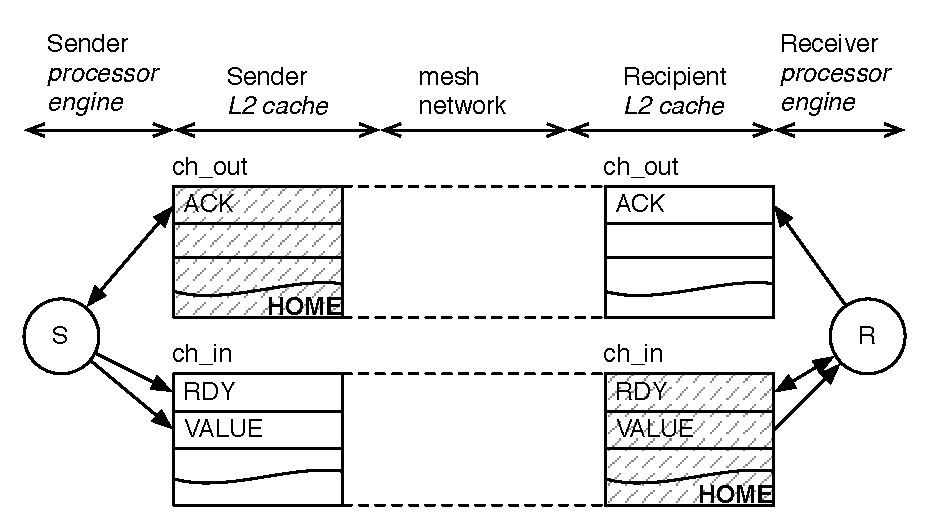
\includegraphics[scale=.5]{cache_sym_sm_fence.pdf}
  \centering
  \caption[Comunicazione simmetrica su memoria condivisa]{Rappresentazione di una comunicazione simmetrica tra i processi $S$ e $R$ con uso della memoria condivisa e gestione ottimizzata della coerenza di cache con strategia Remote Homing per il descrittore di canale}
  \label{fig:cache_sym_sm_fence}
\end{figure}

In conclusione si fa presente che esiste un terzo blocco di cache, usato per il supporto del canale di comunicazione, che contiene i riferimenti alle due parti del descrittore di canale. Tale blocco \`e sempre acceduto in sola lettura, quindi non presenta particolari problemi per le prestazioni e pu\`o essere allocato in uno dei due PE comunicanti con strategia Remote Homing oppure in un terzo PE con strategia Hash-for-Home.

\newpage

\FloatBarrier
\subsubsection{Comunicazione asimmetrica in ingresso}
\label{sct:asymin_sm_rdyack}
Il canale asimmetrico in ingresso \`e visto come costituito da tanti canali simmetrici quanti sono i mittenti. Al fine di ottimizzare le prestazioni non si usa direttamente l'implementazione del canale simmetrico ma si sfruttano comunque i risultati e l'analisi di tale meccanismo, in particolare per quanto riguarda l'allocazione degli oggetti condivisi in cache al fine di garantire la maggiore localit\`a possibile. 

Siano $n$ i processi mittenti del canale, dal punto di vista logico il canale asimmetrico usa $n$ canali simmetrici implementati con il protocollo Rdy-Ack, e perci\`o caratterizzati dal valore della tripla $<Rdy,\; value,\; Ack>$. Come descritto nella sezione \ref{sct:sym_sm_rdyack} i valori di  $Rdy$ e $value$ di un canale simmetrico sono allocati in un blocco che ha per Home il PE che esegue il ricevente mentre $Ack$ ha per Home il il PE che esegue il mittente. Per minimizzare il numero dei blocchi allocati in cache si raggruppa l'insieme dei Rdy e dei valori $\{ <Rdy_i,\; value_i> |\; i \in \{ 1, \dots, n\} \}$ allocandolo come vettore di $n$ coppie $<Rdy,\;value>$ e impostando come Home il PE destinatario, con strategia Remote Homing. I valori di $Ack$ sono invece allocati ciascuno in un blocco che ha per home il PE mittente corrispondente, questo consente la maggior localit\`a possibile. 

Si fa presente che sebbene tale configurazione permetta la massima localit\`a delle informazioni ai PEs, presenta tuttavia l'allocazione nella cache L2 del destinatario di un numero di blocchi che \`e lineare rispetto al numero dei mittenti: si hanno $\frac{2 \cdot 4 \cdot n}{64}$ blocchi necessari a memorizzare l'array di coppie $<Rdy,\;value>$ e $n$ blocchi allocati per le scritture sui flag $Ack$ degli $n$ mittenti. Considerando il caso della comunicazione con il massimo numero (63) di mittenti, si hanno 72 blocchi allocati nel PE destinatario, ovvero uno spazio di 4.5 KB su un totale di 64KB nella cache L2. Dato che siamo interessati a massimizzare le prestazioni si assume che l'uso di tale spazio nella L2 del destinatario non sia problematico per l'applicazione. 

Si osserva che, soprattutto con un numero elevato di mittenti, la sveglia del destinatario sar\`a pi\`u lenta rispetto a quella nel canale simmetrico, infatti l'attesa \`e implementata eseguendo la scansione delle variabili $Rdy$ perci\`o nel caso peggiore \`e necessario effettuare $n$ accessi alla memoria dalla scrittura del valore 1 in un flag $Rdy$ da parte del mittente.

Il descrittore di canale \`e costituito da $n$ riferimenti ai valori di $Ack$ allocati con strategia Remote Homing nei PEs mittenti, e il riferimento alla base del vettore delle coppie $<Rdy, value>$ allocato con strategia Remote Homing nel PE destinatario. Come descritto nella sezione~\ref{sct:specif_meccanismi_intro} il protocollo di comunicazione rimane sosta\-nzialmente invariato rispetto al caso simmetrico, rimane da specificare la politica adottata dal ricevente per selezionare il mittente da cui ricevere tra quelli che hanno inviato un nuovo messaggio. Il supporto della primitiva di ricezione adotta una scansione lineare dell'insieme dei flag $Rdy$ alla ricerca di uno attivo. Ad ogni ricezione viene salvato l'indice del mittente da cui si \`e effettuata la lettura, in modo tale che alla prossima esecuzione della ricezione la scansione dei $Rdy$ si avviata dal mittente successivo. La ricezione \`e quindi non deterministica ed \`e attuata un politica di fairness, sebbene la propriet\`a non sia formalmente soddisfatta. 

Al fine di attuare il protocollo di comunicazione esiste una questione che l'implementazione del supporto della primitiva di invio deve risolvere: conoscere l'identificatore all'interno del canale asimmetrico del mittente che ha eseguito la primitiva. Tale informazione \`e ovviamente indispensabile al protocollo di invio, tra le possibili soluzioni si sono valutate le seguenti due:
\begin{itemize}    
\item la primitiva di invio contiene un terzo parametro, l'identificatore del mittente nel canale, oltre al riferimento al descrittore di canale e al valore del messaggio,
\item ogni mittente usa un proprio descrittore di canale che contiene l'identificatore all'interno del canale, per far ci\`o \`e necessaria una funzione di inizializzazione eseguite da ogni mittente prima dell'avvio della computazione.
\end{itemize}
Si \`e scelta la prima soluzione in quanto anche l'implementazione che sfrutta la UDN verifica lo stesso problema perci\`o \`e assicurata l'uniformit\`a della primitiva di invio nelle due implementazioni del canale asimmetrico. \`E responsabilit\`a dell'utente far si che ogni processo mittente del canale conosca il proprio identificatore univoco all'interno del canale e quindi poter invocare correttamente la primitiva di invio sul canale.
%% 2 * 4 * 64 / 64 + 64 = 8 + 64 = 72 blocchi = 72 * 64 B = 4608 B = 4.5 KB = 1152 word su un totale di 64KB
\begin{figure}[!tb]
  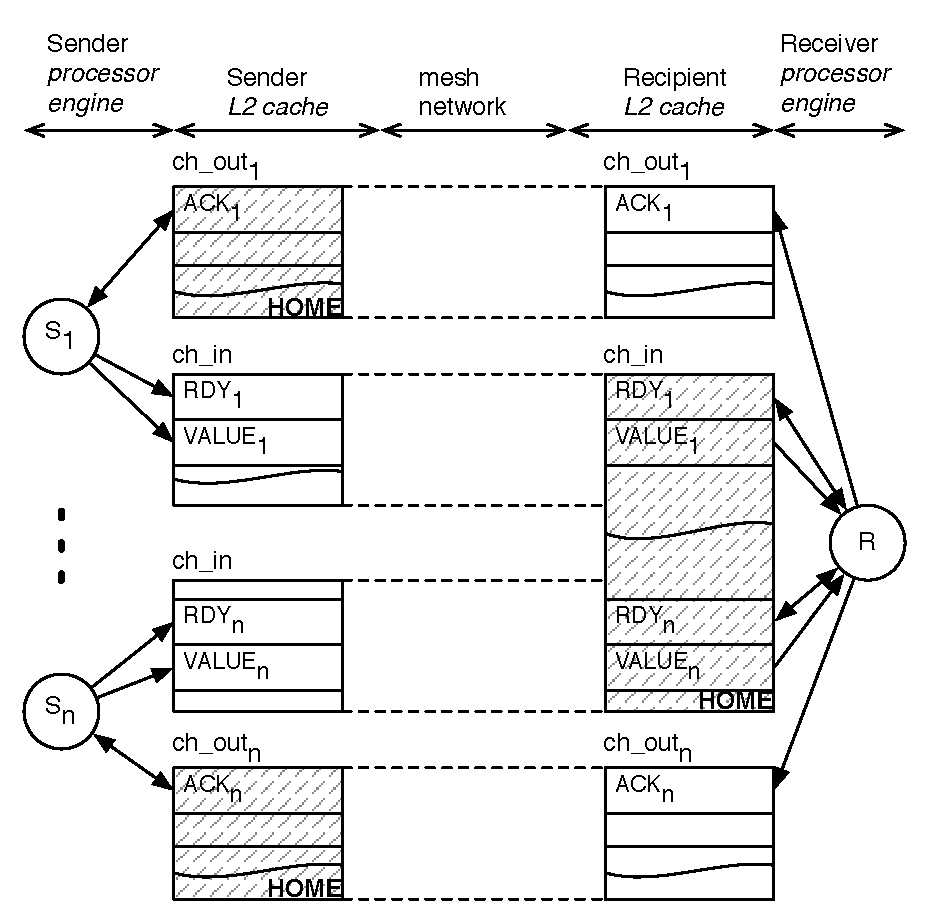
\includegraphics[scale=.5]{cache_asym_sm.pdf}
  \centering
  \caption[Comunicazione asimmetrica su memoria condivisa]{Rappresentazione di una comunicazione asimmetrica tra i processi $\{S_1, \ldots, S_n\}$ e $R$ con uso della memoria condivisa e gestione ottimizzata della coerenza di cache con strategia Remote Homing per il descrittore di canale}
  \label{fig:cache_asym_sm}
\end{figure}

\FloatBarrier
\subsubsection{Comunicazione simmetrica senza barriera di memoria}
\label{sct:sym_sm_nullack}
Nella sezione~\ref{sct:sym_sm_rdyack} si \`e descritta l'implementazione del supporto alla comunicazione simmetrica per mezzo di strutture dati lock-free e, per garantire la correttezza, l'uso della barriera di memoria nel supporto della primitiva di invio. Si propone un'altra possibile implementazione della comunicazione simmetrica con un diverso protocollo che consente il corretto funzionamento con strutture dati lock-free senza l'uso di barriere di memoria. Il protocollo che si va a definire si rif\`a a quello Rdy-Ack, in quanto sono mantenuti gli eventi di sincronizzazione ``messaggio pronto'' (Rdy) e ``messaggio ricevuto'' (Ack). In questo caso l'evento di Rdy non \`e segnalato esplicitamente ma risulta implicito nel cambiamento di valore del canale. Viene infatti definito il valore particolare $\alpha$ che non pu\`o essere assunto dai messaggi trasmessi nel canale e che indica la situazione in cui il canale \`e vuoto. 
Il canale assume valore $\alpha$ all'avvio dell'applicazione e al termine di ogni esecuzione della primitiva di ricezione.
Il flag \verb+Rdy+ \`e eliminato dall'implementazione, il destinatario usa il valore del canale e il valore $\alpha$ per determinare la presenza di un nuovo messaggio, come descritto in codice~\ref{lst:abstr_mem_sym_nullack}. 

Anzitutto si osserva che tale protocollo si applica bene alla nostra implementazione dei canali, in quanto si pu\`o definire, senza perdere di generalit\`a, il valore particolare $\alpha$ come il valore di puntatore ``nullo'': \verb+NULL = (void *) 0+. 
Passando all'analisi della correttezza, la barriera di memoria \`e stata eliminata nella primitiva di invio, in quanto esiste un unico oggetto (il campo \verb+value+) che \`e scritto dal mittente ed \`e acceduto da altri processi.
Nella primitiva di ricezione si hanno invece due oggetti, i campi \verb+value+ e \verb+ack+, che sono scritti dal ricevente ed acceduti dal processo partner. Grazie alla specifica politica di homing di tali oggetti e alla modalit\`a di accesso a questi del processo mittente, l'uso di una memory fence non \`e necessario. Risulta invece sufficiente che il PE che esegue il processo destinatario produca le due scritture nell'ordine specificato. Il campo \verb+value+ ha per Home il PE che esegue il processo ricevente ed \`e acceduto in scrittura dal processo mittente dopo aver letto la variazione di valore del campo \verb+ack+. La prima scrittura \`e quindi locale alla L2 del ricevente, inoltre non ha importanza in che istante diventa visibile agli altri PEs, in quanto l'oggetto scritto (\verb+value+) \`e acceduto in sola scrittura dal mittente. La seconda scrittura \`e una write-through alla L2 del mittente, il quale, una volta letto il nuovo valore pu\`o effettuare una nuova scrittura sul campo \verb+value+ che sicuramente \`e gi\`a stato modificato a \verb+NULL+. Per imporre l'ordinamento delle istruzioni nel PE ricevente si usa l'istruzione \verb+compiler_barrier()+, la quale \`e molto diversa da una barriera di memoria. Il comportamento delle scritture infatti resta asincrono, si \`e solo negato lo spostamento di codice da parte del compilatore, e quindi un ordine diverso di produzione delle due scritture.

\begin{lstlisting}[
        float=t,
        morekeywords={ack, value}, 
        caption={Descrizione astratta del protocollo di comunicazione Null-Ack su memoria condivisa},
        label={lst:abstr_mem_sym_nullack}
]
send(ch_descr, msg) ::
  wait until ch_descr->ack flag is equal to 1;
  reset ch_descr->ack flag to 0;
  copy msg into ch_descr->value entry;

receive(ch_descr) ::
  wait until ch_descr->value is not equal to NULL;
  read the ch_descr->value entry;
  set ch_descr->value to NULL;
  compiler_barrier();
  set ch_descr->ack flag to 1;
\end{lstlisting}
